\documentclass[12pt]{article}
\usepackage{fatec-ti}
\usepackage{url}
\def\UrlBreaks{\do\/\do-}
\usepackage{graphicx,url}
\usepackage[brazil]{babel}
\usepackage[utf8]{inputenc}
\usepackage{longtable}
\usepackage{tabularx}
\usepackage{float}
\usepackage{booktabs}
\usepackage{array}
\usepackage{enumitem}
\sloppy
\graphicspath{{screenshots/}}

\renewcommand{\thesection}{\arabic{section}.}
\renewcommand{\thesubsection}{\arabic{section}.\arabic{subsection}.}
\renewcommand{\figurename}{Figura}
\renewcommand{\tablename}{Tabela}

\newcommand{\foodflowfigure}[3]{
\begin{figure}[H]
    \centering
    \includegraphics[width=#1\textwidth]{#2}
    \caption{#3}
\end{figure}
}

\title{FoodFlow: Plataforma Inteligente para Gestão de Estoques Alimentares e Redução de Desperdício}

\author{Nathan Bandeira Pedrozo\inst{1}, Guilherme Neves\inst{1}, Fernando B. Martins\inst{1}}

\address{Análise e Desenvolvimento de Sistemas -- Faculdade de Tecnologia SENAC Pelotas\\
  Rua Gonçalves Chaves 602 -- 96015-560 -- Pelotas -- RS -- Brazil\\
  \email{\{nathan.bandeira, guilherme.neves, fernando.martins\}@aluno.senacrs.edu.br}
}

\begin{document}

\maketitle

\begin{abstract}
This article presents the development and technical documentation of ``FoodFlow'', a web platform designed to support food inventory management in domestic and professional environments. In this work, we analyze the problem of food waste caused by poor stock visibility, expiration control failures and lack of consumption history. The platform combines pantry management, user collaboration, reports, artificial intelligence, receipt reading, package recognition and price comparison. Based on modern software engineering principles, we examine the system requirements, business rules, architecture, database model, infrastructure and implementation decisions. The analysis shows that FoodFlow goes beyond a simple food list, becoming an integrated decision-support system for food storage, consumption tracking and restocking planning.

\textbf{Keywords:} Web Platform. Food Inventory. Software Architecture. Artificial Intelligence. Next.js. Express. Prisma. PostgreSQL.
\end{abstract}

\begin{resumo}
Este artigo apresenta o desenvolvimento e a documentação técnica do ``FoodFlow'', uma plataforma web criada para apoiar a gestão de estoques alimentares em ambientes domésticos e profissionais. Neste trabalho, analisamos o problema do desperdício de alimentos causado pela baixa visibilidade do estoque, falhas no controle de validade e ausência de histórico de consumo. A plataforma combina gerenciamento de dispensas, colaboração entre usuários, relatórios, inteligência artificial, leitura de notas fiscais, reconhecimento de embalagens e comparação de preços. Com base em princípios modernos de engenharia de software, examinamos os requisitos do sistema, as regras de negócio, a arquitetura, o modelo de banco de dados, a infraestrutura e as decisões de implementação. A análise mostra que o FoodFlow ultrapassa a ideia de uma simples lista de alimentos, tornando-se um sistema integrado de apoio à decisão para armazenamento, consumo e reposição de insumos.

\textbf{Palavras-chave:} Plataforma Web. Estoque Alimentar. Arquitetura de Software. Inteligência Artificial. Next.js. Express. Prisma. PostgreSQL.
\end{resumo}

\section{Introdução}

No contexto da sociedade contemporânea, a gestão de alimentos deixou de ser apenas uma atividade doméstica e passou a fazer parte de uma discussão maior sobre economia, sustentabilidade, organização de processos e redução de desperdícios. Em cozinhas residenciais, restaurantes, cantinas escolares e pequenos estabelecimentos alimentícios, a falta de controle sobre estoque, validade e consumo pode gerar compras duplicadas, vencimento de produtos, perdas financeiras e dificuldade de planejamento.

Neste artigo, analisamos o FoodFlow como uma solução desenvolvida para responder a esse cenário. Nós o compreendemos como uma plataforma web de gestão alimentar que permite ao usuário criar dispensas, cadastrar alimentos, controlar quantidades, registrar uso, visualizar relatórios e colaborar com outras pessoas. A primeira proposta do sistema se aproxima de uma agenda digital de alimentos, mas a implementação atual revela um escopo mais amplo: inteligência artificial, reconhecimento de embalagens, leitura de notas fiscais NFC-e, comparação de preços, geração de documentos, chat entre usuários e monitoramento opcional de temperatura. Essa evolução acompanha a transformação das páginas web tradicionais em aplicações web interativas, baseadas em componentes, estados e comunicação contínua com APIs \cite{chen2019}.

\foodflowfigure{0.95}{01_home.png}{Página inicial do FoodFlow, na qual apresentamos a proposta de controle de estoque simples e inteligente.}

Ao longo deste trabalho, escrevemos em primeira pessoa para evidenciar o processo de análise que realizamos sobre o projeto. A partir da leitura do código-fonte, da documentação interna, das rotas de API, das telas implementadas e do banco de dados, identificamos os principais tópicos técnicos e funcionais que estruturam a aplicação.

\section{Problema, Motivação e Objetivos}

Identificamos como problema central a dificuldade de organizar alimentos em ambientes onde há múltiplos produtos, prazos de validade diferentes, usuários diferentes e necessidade de reposição constante. Quando esse controle é feito de forma manual ou informal, torna-se comum perder a visibilidade do que está disponível, não saber quem utilizou determinado item e não conseguir prever compras futuras.

No caso de pequenos negócios, esse problema se relaciona diretamente à lucratividade, pois cada perda de insumo representa custo operacional. No ambiente doméstico, o impacto aparece no orçamento familiar e no desperdício de alimentos. Em cantinas e restaurantes, a ausência de rastreabilidade também dificulta a prestação de contas e o acompanhamento do consumo.

Com o FoodFlow, buscamos analisar uma solução capaz de:

\begin{itemize}
    \item centralizar o cadastro de alimentos por dispensa;
    \item controlar quantidade, unidade, perecibilidade e validade;
    \item registrar o uso dos insumos por usuário e data;
    \item oferecer relatórios e gráficos para apoiar a tomada de decisão;
    \item automatizar cadastros por câmera, IA e nota fiscal;
    \item apoiar a colaboração entre membros de uma mesma dispensa;
    \item ampliar a experiência por meio de recursos sociais e conversacionais.
\end{itemize}

\section{Metodologia de Análise}

Para elaborar este artigo, nós analisamos o projeto por três dimensões principais: funcional, técnica e infraestrutural. Na dimensão funcional, observamos as telas e fluxos de uso. Na dimensão técnica, examinamos rotas, componentes, banco de dados, integrações e validações. Na dimensão infraestrutural, verificamos dependências, ambiente de execução, serviços externos, banco relacional e possibilidades de implantação. Esse processo se aproxima da lógica de Desenvolvimento de Novos Produtos (NPD), na qual a compreensão do problema, a validação do MVP e a organização dos requisitos reduzem riscos de desenvolvimento \cite{falahat2024}.

Também seguimos parâmetros comuns em artigos de desenvolvimento de software, como fundamentação teórica, levantamento de requisitos, regras de negócio, decisões arquiteturais, modelagem de dados e documentação visual do sistema. Essa organização foi escolhida porque permite demonstrar não apenas o que o FoodFlow faz, mas também como a solução foi construída e quais escolhas técnicas sustentam suas funcionalidades.

\section{Fundamentação Teórica e Trabalhos Relacionados}

Nesta seção, realizamos uma análise bibliográfica voltada às tecnologias e conceitos que fundamentam o FoodFlow. Assim como no artigo de referência, organizamos a fundamentação por camadas técnicas e por decisões de produto, pois isso permite justificar a escolha das tecnologias e relacioná-las diretamente aos requisitos do sistema.

\subsection{Fundamentação Teórica}

\subsubsection{Tecnologias de Front-end: React e Next.js}

A construção de aplicações web modernas baseia-se na separação de responsabilidades entre cliente e servidor. Para a interface do FoodFlow, identificamos o uso de React por meio do Next.js. O React consolidou a construção de interfaces a partir de componentes reutilizáveis, estados e renderização declarativa, o que facilita manutenção e evolução visual \cite{chen2019}. Essa abordagem é coerente com o FoodFlow, pois a aplicação possui várias telas e modais reutilizáveis: cadastro, login, perfil, dispensa, relatórios, chat, leitura de nota fiscal e reconhecimento de embalagem.

O Next.js, por sua vez, oferece roteamento estruturado, organização por páginas, otimizações de build e recursos adequados para aplicações React em produção \cite{prabakar2025}. No FoodFlow, o uso de Next.js permite organizar o frontend por rotas como \texttt{/login}, \texttt{/register}, \texttt{/perfil}, \texttt{/dispensa/[id]}, \texttt{/relatorios/[id]} e \texttt{/precos}. Essa estrutura torna o sistema mais previsível para manutenção e facilita a expansão do produto.

\subsubsection{Tecnologias de Back-end: Express.js e APIs REST}

No lado do servidor, analisamos uma API construída com Express.js e TypeScript. O Express permite organizar endpoints, middlewares e rotas de forma simples, o que é adequado para MVPs e sistemas com domínios bem separados \cite{express}. Embora o artigo de exemplo utilize Django como backend, no FoodFlow identificamos uma escolha mais próxima do ecossistema JavaScript/TypeScript, mantendo a mesma linguagem-base no frontend e no backend.

Essa decisão reduz a troca de contexto entre camadas e facilita o desenvolvimento full-stack. As rotas do FoodFlow são separadas por domínio, como clientes, login, dispensa, alimentos, mensagens, amizades, convites, IA, reconhecimento de produtos e notas fiscais. Essa modularização atende ao princípio de manutenibilidade descrito por Pressman e Maxim e por Sommerville, no qual sistemas evolutivos devem favorecer separação de responsabilidades e baixo acoplamento \cite{pressman,sommerville}.

\subsubsection{Persistência de Dados: Prisma e PostgreSQL}

Para persistência, identificamos o uso de PostgreSQL com Prisma ORM. O Prisma permite modelar entidades, relações, enums, índices e migrações em um schema declarativo \cite{prisma}. Essa abordagem reduz a necessidade de consultas SQL manuais e facilita a evolução do banco de dados. No FoodFlow, isso é importante porque o domínio envolve várias relações: usuários possuem dispensas, dispensas possuem alimentos, usuários registram uso de alimentos, amigos trocam mensagens e notas fiscais possuem itens.

A escolha por banco relacional é coerente com o tipo de dado manipulado. O sistema precisa garantir consistência entre estoque e histórico de uso, além de preservar relações entre compras, usuários e dispensas. Nesse sentido, o PostgreSQL é adequado por oferecer integridade relacional, transações e suporte a tipos estruturados.

\subsubsection{Arquitetura: Monolito Modular e Microsserviços}

A arquitetura do FoodFlow se aproxima de um monolito modular dividido em frontend, backend e banco de dados. O backend não está fragmentado em microsserviços; em vez disso, concentra as rotas em uma única aplicação Express. Essa decisão é adequada para um MVP, pois aplicações monolíticas costumam ser mais simples de testar, implantar, depurar e monitorar do que sistemas distribuídos \cite{blinowski2022}.

Pesquisas comparativas apontam que microsserviços podem trazer escalabilidade e independência de implantação, mas também aumentam a complexidade operacional, a comunicação entre processos e os custos de observabilidade \cite{blinowski2022}. Para o estágio atual do FoodFlow, a organização modular dentro de uma mesma API parece suficiente e evita complexidade prematura.

\subsubsection{Inteligência Artificial e Automação}

O FoodFlow também se apoia em serviços de IA generativa. A integração com Google Gemini permite implementar assistente culinário, assistente inteligente da dispensa e reconhecimento de embalagens \cite{gemini}. Nesse ponto, a IA não é tratada apenas como elemento conversacional, mas como mecanismo de automação para reduzir esforço manual. A câmera do navegador, por meio da API \texttt{getUserMedia()}, complementa esse fluxo ao permitir captura de imagens diretamente pela interface web \cite{mdn}.

\subsubsection{Desenvolvimento de Novos Produtos e MVP}

Do ponto de vista de produto, analisamos o FoodFlow como um MVP expandido. A literatura sobre NPD destaca que produtos digitais precisam validar rapidamente a proposta de valor, compreender as necessidades do usuário e reduzir riscos de desenvolvimento \cite{falahat2024}. O FoodFlow atende a essa lógica ao partir de uma dor concreta: dificuldade de controlar alimentos, validade e consumo. A evolução para IA, nota fiscal e comparação de preços indica uma expansão incremental sobre uma base funcional já validável.

\subsection{Trabalhos Relacionados}

Para posicionar o FoodFlow, analisamos sistemas similares. O primeiro é o \textbf{Grocy}, uma solução open-source voltada ao gerenciamento doméstico de despensa, validade, compras e consumo. O FoodFlow se aproxima do Grocy no controle de alimentos, mas se diferencia pela camada social, chat entre usuários, reconhecimento de embalagens e importação de nota fiscal.

O segundo sistema relacionado é o \textbf{MarketMan}, voltado à gestão profissional de estoque em restaurantes. O FoodFlow se aproxima desse tipo de ferramenta ao oferecer relatórios, histórico de consumo e apoio a decisões de compra, mas mantém uma proposta mais acessível para uso doméstico, escolar e de pequenos negócios.

Também podemos aproximar o FoodFlow de sistemas de comparação de preços e apps de lista de compras. Entretanto, sua característica diferencial está na integração dos fluxos: o usuário cadastra alimentos, registra uso, importa compras, compara preços e planeja reposição dentro de uma mesma plataforma.

\section{Levantamento de Requisitos}

Ao analisar o sistema, identificamos requisitos funcionais e não funcionais. Entre os requisitos funcionais, destacamos:

\begin{itemize}
    \item permitir cadastro e autenticação de usuários;
    \item criar e gerenciar dispensas;
    \item cadastrar, editar, remover e listar alimentos;
    \item registrar uso de alimentos e atualizar o estoque;
    \item gerar relatórios e gráficos;
    \item permitir convites para membros de uma dispensa;
    \item manter sistema de amizades e mensagens;
    \item sugerir receitas e responder dúvidas por IA;
    \item reconhecer embalagens por imagem;
    \item ler notas fiscais NFC-e e importar itens;
    \item comparar preços entre mercados;
    \item sugerir reposição com base nas datas de validade.
\end{itemize}

Entre os requisitos não funcionais, identificamos responsividade, segurança, manutenibilidade, escalabilidade, compatibilidade com navegadores modernos e disponibilidade de serviços externos. Esses requisitos são importantes porque o sistema depende de interações móveis, câmera, API externa de IA, banco remoto e dados compartilhados entre usuários.

\subsection{Diagrama de Casos de Uso}

Para representar visualmente as interações entre os atores e o sistema, elaboramos o diagrama de casos de uso da Figura \ref{fig:casosuso}. Nele, distinguimos quatro atores humanos principais: visitante, usuário autenticado, proprietário da dispensa e membro da dispensa. Também representamos serviços externos que participam de fluxos específicos, como Google Gemini, NFC-e/SEFAZ e ThingSpeak.

\begin{figure}[H]
    \centering
    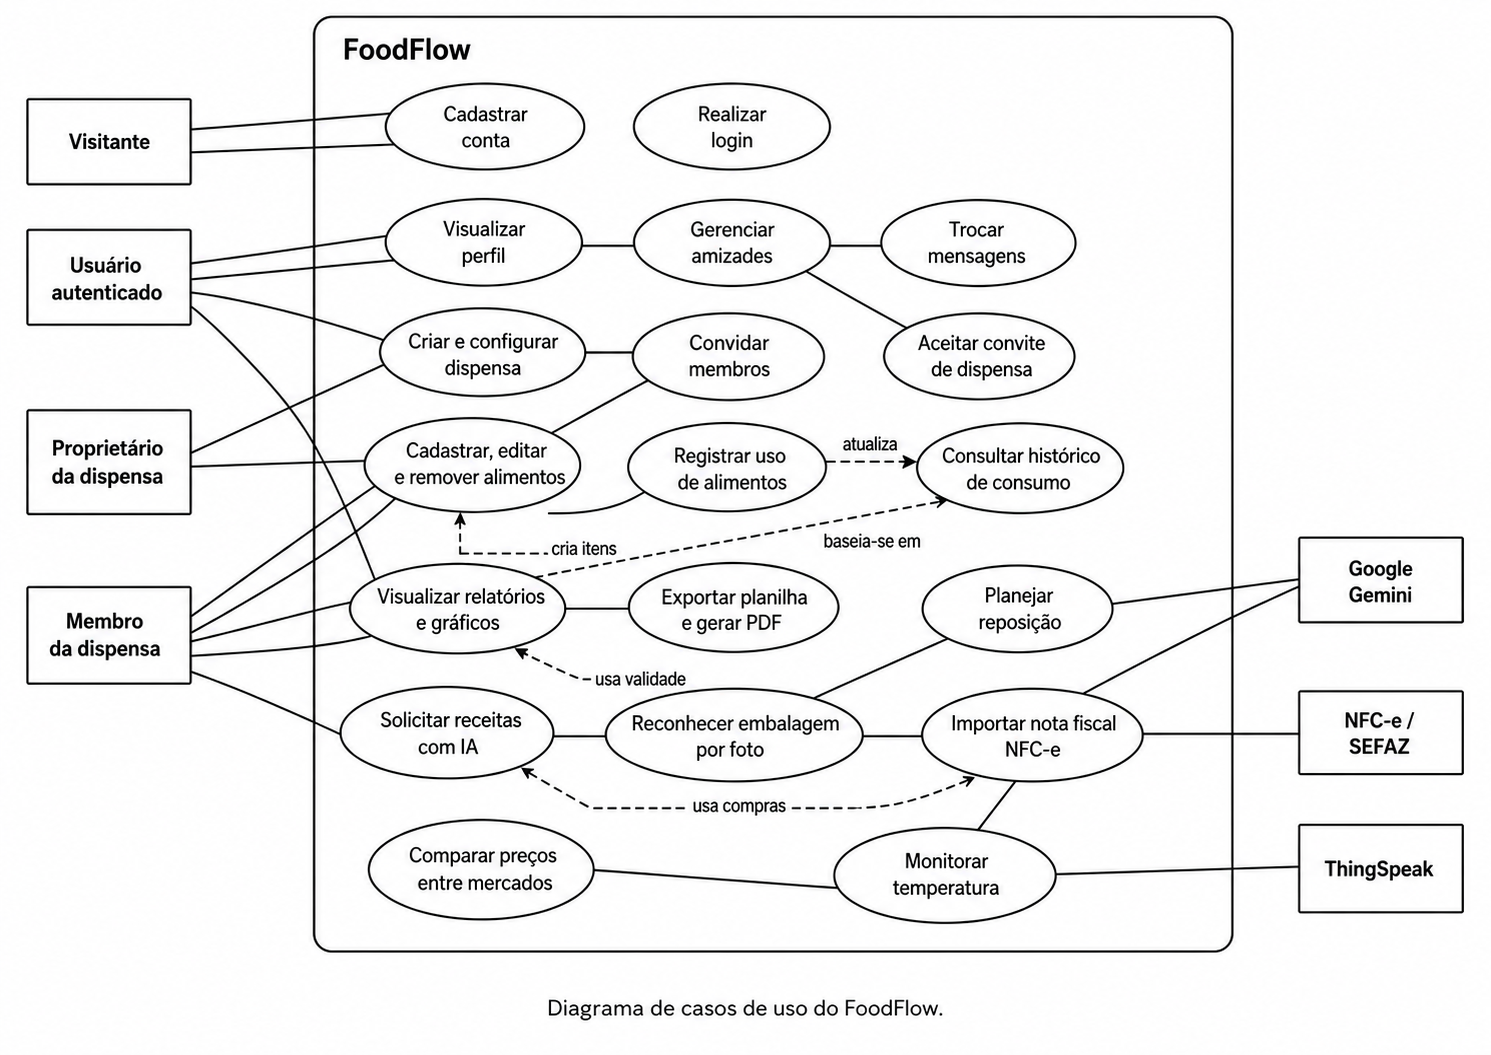
\includegraphics[width=0.98\textwidth]{18_diagrama_caso_uso.png}
    \caption{Diagrama de casos de uso do FoodFlow.}
    \label{fig:casosuso}
\end{figure}

\section{Regras de Negócio}

As regras de negócio do FoodFlow definem como o sistema deve se comportar em situações específicas. Identificamos as seguintes regras principais:

\begin{itemize}
    \item um usuário precisa estar autenticado para acessar as funcionalidades internas;
    \item uma dispensa pertence a um usuário proprietário, mas pode possuir membros convidados;
    \item um alimento deve estar associado a uma dispensa;
    \item o registro de uso não deve permitir quantidade maior do que a disponível;
    \item ao registrar uso, o sistema deve reduzir a quantidade do alimento e criar histórico;
    \item convites de amizade e de dispensa podem ser aceitos ou rejeitados;
    \item uma nota fiscal já importada não deve ser duplicada na mesma dispensa;
    \item produtos reconhecidos por IA devem ser revisados antes da persistência;
    \item itens próximos do vencimento devem receber prioridade nas análises de reposição;
    \item a comparação de preços deve agrupar nomes semelhantes para evitar duplicidade visual.
\end{itemize}

Essas regras reforçam que o FoodFlow não é apenas uma interface de cadastro. Ele possui lógica de domínio para controlar estoque, consumo, colaboração e tomada de decisão.

\section{Arquitetura Técnica do Sistema}

A arquitetura do FoodFlow é organizada em três camadas principais: frontend, backend e banco de dados. No frontend, usamos Next.js, React, TypeScript, Tailwind CSS, componentes de interface e bibliotecas como Recharts para gráficos. No backend, identificamos uma API Express.js em TypeScript, com Prisma ORM, validação por Zod, autenticação JWT e integração com Google Gemini. Na persistência, o sistema usa PostgreSQL.

\begin{itemize}
    \item \textbf{Frontend}: responsável pela experiência do usuário, telas, modais, gráficos, câmera e chamadas à API.
    \item \textbf{Backend}: responsável por regras de negócio, validações, autenticação, integrações externas e persistência.
    \item \textbf{Banco de dados}: responsável por armazenar usuários, dispensas, alimentos, histórico de uso, mensagens, amizades, convites e notas fiscais.
\end{itemize}

O backend centraliza as rotas no arquivo principal da aplicação e organiza cada domínio em um arquivo próprio. Essa decisão facilita a manutenção, pois mudanças em alimentos, notas fiscais ou mensagens tendem a ficar localizadas em módulos específicos.

\section{Análise de Infraestrutura}

Na análise de infraestrutura, observamos que o projeto foi pensado para execução local em dois serviços principais: frontend em \texttt{localhost:3000} e backend em \texttt{localhost:3001}. O banco de dados é acessado por meio da variável \texttt{DATABASE\_URL}, e as integrações de IA usam chaves em variáveis de ambiente, como \texttt{GEMINI\_API\_KEY} e \texttt{GOOGLE\_API\_KEY}. Essa separação operacional segue uma arquitetura simples de implantação, adequada a MVPs, porque reduz a complexidade inicial quando comparada a ambientes de microsserviços \cite{blinowski2022}.

O frontend depende da variável \texttt{NEXT\_PUBLIC\_URL\_API} para localizar o backend. Essa separação permite executar a interface e a API em processos independentes, o que favorece escalabilidade e implantação em ambientes distintos. Em um cenário de produção, o frontend poderia ser hospedado em uma plataforma especializada para aplicações Next.js, enquanto o backend poderia ser implantado em um serviço de aplicação Node.js. Essa estratégia é compatível com as vantagens de distribuição e otimização descritas para aplicações Next.js modernas \cite{prabakar2025}. Também observamos uma estrutura Android com Capacitor, o que indica a intenção de transformar a aplicação web em uma experiência mobile. Essa decisão é coerente com funcionalidades como câmera, QR code e uso em cozinhas, onde o celular costuma ser mais acessível que um computador.

Em termos de serviços externos, identificamos quatro pontos de dependência:

\begin{itemize}
    \item banco PostgreSQL para persistência dos dados;
    \item Google Gemini para recursos de inteligência artificial;
    \item API ThingSpeak para monitoramento opcional de temperatura;
    \item páginas de NFC-e/SEFAZ para leitura de notas fiscais.
\end{itemize}

Essa infraestrutura amplia as capacidades do sistema, mas também cria riscos. Se a API de IA estiver indisponível, o reconhecimento de embalagens e os assistentes podem falhar. Se a página da nota fiscal estiver lenta ou bloquear consultas, a importação automática pode ser prejudicada. Por isso, recomendamos que versões futuras tenham estratégias de fallback manual, logs de erro, limites de requisição e mensagens claras para o usuário.

\section{Modelagem do Banco de Dados}

O banco de dados foi modelado em torno das entidades que sustentam o domínio alimentar e social do sistema. Entre os modelos principais, identificamos \texttt{Usuario}, \texttt{Dispensa}, \texttt{Alimentos}, \texttt{UsoAlimento}, \texttt{UsuarioNaDispensa}, \texttt{Mensagem}, \texttt{Amizade}, \texttt{FriendRequest}, \texttt{DispensaInvite}, \texttt{NotaFiscalCompra} e \texttt{NotaFiscalItem}.

\foodflowfigure{0.98}{00_diagrama_banco_dados.png}{Diagrama relacional do banco de dados do FoodFlow, representando usuários, dispensas, alimentos, mensagens, amizades, convites e notas fiscais.}

Ao observar o diagrama, percebemos que a \texttt{Dispensa} é a entidade central do domínio. Ela se relaciona com alimentos, membros, histórico de uso e notas fiscais. O modelo \texttt{UsoAlimento} permite rastrear consumo e associar cada movimentação a um usuário. Já os modelos \texttt{Mensagem}, \texttt{Amizade} e \texttt{FriendRequest} sustentam a camada social do sistema. A presença de \texttt{NotaFiscalCompra} e \texttt{NotaFiscalItem} amplia o banco para análise de compras e comparação de preços.

\section{Funcionalidades Implementadas}

\subsection{Autenticação, Cadastro e Perfil}

No fluxo de autenticação, analisamos o cadastro de usuários, o login e a persistência da sessão. O backend valida os dados, aplica hash de senha com bcrypt e emite um token JWT no login. No frontend, o usuário autenticado acessa a página de perfil, onde visualiza suas dispensas e amigos.

\foodflowfigure{0.82}{02_login.png}{Tela de login utilizada para autenticar o usuário.}

\foodflowfigure{0.82}{03_cadastro.png}{Tela de cadastro de novos usuários.}

\foodflowfigure{0.95}{04_perfil_dispensas_amigos.png}{Perfil com amigos e dispensas vinculadas ao usuário.}

\subsection{Gestão de Dispensa e Estoque}

Na gestão da dispensa, identificamos o núcleo operacional do sistema. Nessa tela, o usuário visualiza os alimentos cadastrados, pesquisa itens, acessa gráficos, registra uso, adiciona membros, abre o assistente e aciona automações como foto e nota fiscal.

\foodflowfigure{0.95}{05_dispensa_estoque.png}{Tela principal da dispensa com alimentos cadastrados, membros e atalhos de operação.}

O cadastro manual de alimento usa um modal com campos de nome, quantidade, unidade, perecibilidade e validade. Esse fluxo é importante porque serve como fallback quando a IA, a câmera ou a leitura fiscal não estão disponíveis.

\foodflowfigure{0.95}{08_modal_adicionar_item.png}{Modal de cadastro manual de alimentos na dispensa.}

\subsection{Registro de Uso e Rastreabilidade}

O registro de uso permite informar quanto foi consumido de cada item. No backend, essa operação é transacional: primeiro o sistema valida se o alimento pertence à dispensa, depois verifica se existe quantidade suficiente, atualiza o saldo e registra a movimentação. Com isso, conseguimos rastrear quem usou, quando usou e quanto usou.

\foodflowfigure{0.95}{06_dispensa_registrar_uso.png}{Formulário para registrar o uso de alimentos e atualizar o estoque.}

\subsection{Relatórios e Gráficos}

Os relatórios são uma das partes mais importantes da plataforma, pois transformam dados operacionais em informação para tomada de decisão. A tela apresenta histórico de utilização, gráfico de consumo, busca, exportação e geração de documento.

\foodflowfigure{0.95}{12_relatorios_historico_consumo.png}{Página de relatórios com histórico de utilização e gráfico de consumo.}

Também analisamos o gráfico de distribuição do estoque, que apresenta visualmente a proporção dos alimentos cadastrados. Essa representação facilita a leitura do estoque e ajuda a identificar itens em maior volume.

\foodflowfigure{0.75}{07_dispensa_grafico_distribuicao.png}{Gráfico de distribuição dos alimentos no estoque.}

Além disso, o sistema permite gerar um documento em PDF a partir do histórico, com título, organização, observações e imagem opcional. Essa funcionalidade aproxima o FoodFlow de ambientes institucionais, como escolas e cantinas.

\foodflowfigure{0.95}{14_modal_gerar_documento.png}{Gerador de documento do histórico da dispensa.}

\subsection{Assistentes de Inteligência Artificial}

O FoodFlow possui dois usos principais de IA. O primeiro é o assistente culinário, que responde perguntas sobre receitas e preparo de alimentos. O segundo é o assistente da dispensa, capaz de interpretar comandos de linguagem natural para adicionar itens, registrar uso e orientar o usuário.

\foodflowfigure{0.95}{11_assistente_culinario.png}{Assistente culinário com interface conversacional.}

Ao analisar essa funcionalidade, entendemos que a IA reduz atrito de uso, pois o usuário pode interagir por texto em vez de navegar por formulários. Essa abordagem é especialmente útil para tarefas rápidas, como registrar consumo ou obter sugestões de preparo.

\subsection{Reconhecimento de Embalagens}

No reconhecimento de embalagens, o sistema usa câmera, imagem em base64 e Google Gemini Vision para extrair dados de um produto. O fluxo previsto identifica nome, marca, peso, unidade, validade, ingredientes, nutrientes, código de barras e nível de confiança. Antes de salvar, o usuário revisa os dados, evitando que a automação cadastre informações incorretas.

\foodflowfigure{0.95}{09_modal_reconhecimento_embalagem.png}{Modal de reconhecimento de embalagem por câmera.}

Essa função é relevante porque acelera o cadastro e reduz erros manuais. Tecnicamente, ela depende de permissão de câmera no navegador, envio de imagem ao backend e tratamento de resposta JSON da IA.

\subsection{Leitura de Nota Fiscal NFC-e}

Outra automação identificada é a leitura de nota fiscal NFC-e. O usuário pode ler um QR code pela câmera, enviar uma imagem ou colar a URL/texto da nota. O backend interpreta a nota, extrai itens e classifica quais produtos são alimentos. Os itens alimentícios podem ser enviados diretamente para a dispensa.

\foodflowfigure{0.95}{10_modal_leitor_nota_fiscal.png}{Leitor de nota fiscal NFC-e com captura por câmera, upload e campo manual.}

Essa funcionalidade conecta o FoodFlow ao processo real de compra. Em vez de cadastrar manualmente item por item, o usuário pode aproveitar os dados fiscais da compra para alimentar o estoque.

\subsection{Comparação de Preços}

Com base nos itens importados por nota fiscal, o sistema compara preços entre mercados. Para isso, normaliza nomes, remove termos pouco relevantes e agrupa produtos semelhantes. O resultado mostra menor preço, economia possível e mercados associados.

\foodflowfigure{0.95}{15_comparacao_precos.png}{Tela de comparação de preços entre mercados.}

Essa funcionalidade amplia o escopo do sistema. Nós deixamos de analisar apenas o controle interno de estoque e passamos a observar uma camada de inteligência de compra, que pode ajudar o usuário a decidir onde repor insumos.

\subsection{Planejamento de Reposição}

O planejamento de reposição analisa datas de validade e calcula janelas de urgência. O sistema diferencia itens vencidos, críticos, próximos do vencimento e itens com maior folga. A partir disso, sugere quando repor e indica fornecedores por categoria.

\foodflowfigure{0.95}{13_modal_reposicao.png}{Modal de planejamento de reposição com itens críticos e fornecedores sugeridos.}

Mesmo sendo baseado em heurísticas, esse recurso é importante porque transforma dados de validade em recomendação prática. Assim, o usuário não apenas consulta o estoque, mas recebe apoio para decidir o próximo movimento.

\subsection{Amizades, Convites e Chat}

O FoodFlow também possui uma camada social. Identificamos busca de usuários, solicitações de amizade, listagem de contatos, mensagens e chat. Esses recursos tornam a gestão mais colaborativa, especialmente quando várias pessoas participam da mesma rotina alimentar.

\foodflowfigure{0.95}{16_amigos.png}{Tela de amizades e contatos do usuário.}

\foodflowfigure{0.95}{17_chat_usuarios.png}{Chat entre usuários da plataforma.}

\section{Endpoints e Integrações}

A API do FoodFlow é organizada por grupos de endpoints. A Tabela \ref{tab:endpoints} sintetiza os principais módulos.

\begin{table}[H]
\centering
\caption{Principais grupos de endpoints identificados no backend.}
\label{tab:endpoints}
\begin{tabular}{p{4cm}p{9cm}}
\toprule
\textbf{Grupo} & \textbf{Exemplos de endpoints} \\
\midrule
Usuários & \texttt{GET/POST /clientes}, \texttt{POST /clientes/login} \\
Dispensas & \texttt{GET /dispensa/:id}, \texttt{POST /dispensa}, \texttt{DELETE /dispensa/:id} \\
Alimentos & \texttt{GET /alimentos/dispensa/:id/alimentos}, \texttt{POST /alimentos/dispensa/:id/alimentos} \\
Uso e relatórios & \texttt{POST /alimentos/relatorio}, \texttt{GET /alimentos/relatorio/:dispensaId} \\
Amizades & \texttt{GET /amigos}, \texttt{POST /friendRequests}, \texttt{POST /friendRequests/:id/accept} \\
Mensagens & \texttt{POST /mensagens}, \texttt{GET /mensagens/conversa/:destinatarioId} \\
Convites & \texttt{POST /dispensaInvites}, \texttt{POST /dispensaInvites/:id/accept} \\
IA & \texttt{POST /gemini}, \texttt{POST /geminiPantry} \\
Reconhecimento & \texttt{POST /productRecognition/analyze}, \texttt{POST /productRecognition/create} \\
Notas fiscais & \texttt{POST /notasFiscais/analisar}, \texttt{POST /notasFiscais/importar}, \texttt{GET /notasFiscais/comparacao} \\
\bottomrule
\end{tabular}
\end{table}

Essa divisão reforça a modularidade do backend e facilita a manutenção por domínio.

\section{Segurança e Validação}

Na análise de segurança, identificamos pontos positivos e pontos de melhoria. Entre os pontos positivos, destacamos o uso de bcrypt para senhas, JWT para autenticação, Zod para validação de entrada, Prisma ORM para acesso ao banco e middleware de verificação de token em rotas sensíveis.

Também observamos verificações de permissão em fluxos como mensagens, solicitações de amizade, convites de dispensa e exclusão de produtos reconhecidos. No entanto, algumas rotas ainda podem ser fortalecidas com autenticação e autorização mais consistentes. Recomendamos que todas as leituras e alterações ligadas a uma dispensa validem se o usuário é proprietário ou membro autorizado.

\section{Resultados e Discussão}

A partir da análise, concluímos que o FoodFlow se comporta como um MVP avançado. Ele não se limita ao cadastro de alimentos, pois integra estoque, relatórios, colaboração, IA, leitura fiscal, comparação de preços e planejamento de reposição. Essa combinação cria valor porque conecta três momentos do ciclo alimentar: entrada de produtos, uso dos produtos e decisão de reposição.

Do ponto de vista técnico, o projeto demonstra boa separação entre camadas e possui uma base relacional coerente com o domínio. Do ponto de vista funcional, as telas capturadas mostram que o sistema oferece fluxos suficientes para uso real em pequena escala. Do ponto de vista de infraestrutura, a aplicação depende de serviços externos importantes, o que exige atenção em produção.

\section{Limitações e Trabalhos Futuros}

Apesar do escopo amplo, identificamos limitações que podem orientar trabalhos futuros:

\begin{itemize}
    \item padronizar autorização em todas as rotas de dispensa;
    \item criar testes automatizados para backend e frontend;
    \item melhorar tratamento de falhas em IA e NFC-e;
    \item revisar normalização de unidades de medida;
    \item ampliar classificação de alimentos em notas fiscais;
    \item integrar bases externas, como Open Food Facts;
    \item consolidar o fluxo mobile com Capacitor;
    \item revisar textos e encoding de dados antigos;
    \item criar uma política clara para usuários gratuitos e premium;
    \item adicionar observabilidade, logs estruturados e métricas de uso.
\end{itemize}

\section{Conclusão}

Neste artigo, apresentamos e analisamos tecnicamente o FoodFlow, uma plataforma web para gestão de estoques alimentares. Ao longo da análise, identificamos que o sistema resolve um problema prático de organização, validade, consumo e reposição de alimentos. Também mostramos que sua arquitetura combina frontend em Next.js, backend em Express, banco PostgreSQL via Prisma e integrações externas para IA, câmera, nota fiscal e temperatura.

Concluímos que o FoodFlow tem potencial para uso doméstico, escolar e profissional, especialmente em contextos que exigem rastreabilidade e redução de desperdícios. A principal contribuição do projeto está em transformar um controle simples de alimentos em uma plataforma de apoio à decisão, capaz de registrar dados, interpretar consumo, automatizar entradas e sugerir ações futuras.

\begin{thebibliography}{12}

\bibitem[Blinowski et al. 2022]{blinowski2022}
Blinowski, G., Ojdowska, A., and Przyby\l{}ek, A. (2022). Monolithic vs. microservice architecture: A performance and scalability evaluation. {\em IEEE Access}, 10:20357--20374.

\bibitem[Chen et al. 2019]{chen2019}
Chen, S., Thaduri, U. R., and Ballamudi, V. K. R. (2019). Front-end development in React: An overview. {\em Engineering International}, 7(2):117--126.

\bibitem[Express 2026]{express}
Express (2026). Express.js routing guide. Disponível em: \url{https://expressjs.com/en/guide/routing/}. Acesso em: 26 jun. 2026.

\bibitem[Falahat et al. 2024]{falahat2024}
Falahat, M., Chong, S. C., and Liew, C. (2024). Navigating new product development: Uncovering factors and overcoming challenges for success. {\em Heliyon}, 10(2):e23763.

\bibitem[Google 2026]{gemini}
Google (2026). Gemini API documentation. Disponível em: \url{https://ai.google.dev/gemini-api/docs}. Acesso em: 26 jun. 2026.

\bibitem[MDN 2026]{mdn}
Mozilla Developer Network (2026). MediaDevices: getUserMedia() method. Disponível em: \url{https://developer.mozilla.org/en-US/docs/Web/API/MediaDevices/getUserMedia}. Acesso em: 26 jun. 2026.

\bibitem[Prabakar et al. 2025]{prabakar2025}
Prabakar, S., Logeshwari, S., Gokulvikram, T., Prasad, J. D., Kumar, K. R., and Sarvesh, J. A. (2025). E-commerce website using Next.js. {\em International Journal of Scientific Research in Engineering and Management (IJSREM)}, 9(4):1--15.

\bibitem[Pressman and Maxim 2016]{pressman}
Pressman, R. S. and Maxim, B. R. (2016). {\em Engenharia de Software: uma abordagem profissional}. 8. ed. Porto Alegre: AMGH.

\bibitem[Prisma 2026]{prisma}
Prisma (2026). Prisma documentation. Disponível em: \url{https://www.prisma.io/docs}. Acesso em: 26 jun. 2026.

\bibitem[Sommerville 2019]{sommerville}
Sommerville, I. (2019). {\em Engenharia de Software}. 10. ed. São Paulo: Pearson.

\end{thebibliography}

\end{document}
